\documentclass[12pt]{scrartcl}
\usepackage[hagavi]{azzam}

% Excircle - Modul (gabungan Materi dan Soal Latihan)
% Materi diadaptasi dari Modul Pra-OSP Excircle (Azzam dan Akeyla),
% `3 Geometri/OrtikEx .../OrtikEx_Materi.tex`, dan
% `3 Geometri/Pelatda OSN SMA 2026 10 September 2026.tex`
% (ditulis ulang dengan contoh pengerjaan tiap blok teori).
% Soal Latihan dari ketiga sumber itu dan Helvethia
% (esai OSP/OSN, EMC, JJMO, dan kontes lain).
% _Solusi tetap terpisah.
% Sumber tiap soal latihan dimunculkan di PDF sebagai \item (Sumber); komentar menyimpan detail lengkap.

\title{Excircle - Modul}
\date{20 November 2026}

\begin{document}
\maketitle

\renewcommand*\contentsname{Daftar Isi}
\tableofcontents

\newpage

\part*{Materi}
\section{Definisi dan Garis Bagi}

\begin{definition}
Diberikan segitiga $ABC$.
\istilah{Lingkaran singgung luar}{excircle} di hadapan $A$,
disebut $A$-excircle, adalah lingkaran yang menyinggung segmen $BC$
serta perpanjangan sisi $AB$ (melewati $B$) dan perpanjangan sisi $AC$
(melewati $C$). Pusatnya disebut $A$-excenter dan dinotasikan $I_A$.
Definisi $B$-excircle dan $C$-excircle analog.
\end{definition}

\begin{example}
Gambarlah $A$-excircle dari segitiga $ABC$ beserta ketiga titik
singgungnya.
\end{example}
\begin{proof}[Solusi]
\begin{center}
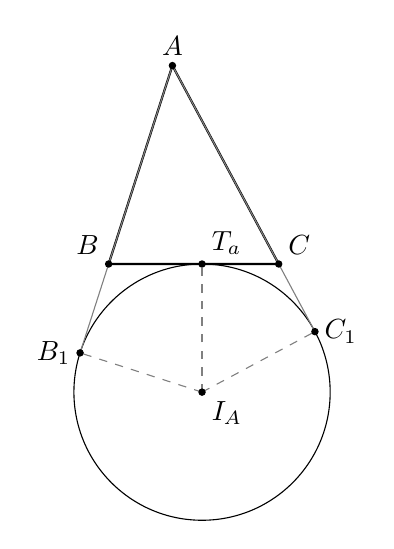
\begin{tikzpicture}[scale=0.9]
    \coordinate (A) at (-0.3,2.8);
    \coordinate (B) at (-1.2,0);
    \coordinate (C) at (1.2,0);
    \coordinate (Ia) at (0.118,-1.808);
    \coordinate (X) at (0.118,0);
    \coordinate (B1) at (-1.603,-1.254);
    \coordinate (C1) at (1.711,-0.954);
    \draw (Ia) circle (1.808);
    \draw[thick] (A) -- (B) -- (C) -- cycle;
    \draw[gray] (A) -- (B1);
    \draw[gray] (A) -- (C1);
    \draw[gray,dashed] (Ia) -- (X);
    \draw[gray,dashed] (Ia) -- (B1);
    \draw[gray,dashed] (Ia) -- (C1);
    \fill (A) circle (1.5pt);
    \fill (B) circle (1.5pt);
    \fill (C) circle (1.5pt);
    \fill (Ia) circle (1.5pt);
    \fill (X) circle (1.5pt);
    \fill (B1) circle (1.5pt);
    \fill (C1) circle (1.5pt);
    \node[above] at (A) {$A$};
    \node[above left] at (B) {$B$};
    \node[above right] at (C) {$C$};
    \node[below right] at (Ia) {$I_A$};
    \node[above right] at (X) {$T_a$};
    \node[left] at (B1) {$B_1$};
    \node[right] at (C1) {$C_1$};
\end{tikzpicture}
\end{center}
Lingkaran menyinggung segmen $BC$ di $T_a$
serta perpanjangan $AB$ dan $AC$ di $B_1$ dan $C_1$.
\end{proof}

\begin{fact}
Notasi $a = BC$, $b = CA$, $c = AB$, incenter $I$,
dan $I_A, I_B, I_C$ para excenter.
\begin{enumerate}
    \item $I_A$ adalah perpotongan garis bagi dalam sudut $A$
    dengan garis bagi luar sudut $B$ dan $C$ (dan siklis).
    \item \textbf{Teorema garis bagi luar.}
    Garis bagi luar sudut $A$ memotong garis $BC$ di $P$ dengan
    \[ \frac{PB}{PC} = \frac{AB}{AC}, \]
    dengan $P$ di luar segmen $BC$, di sisi $B$ jika $AB < AC$.
    \item $I_A, C, I_B$ segaris (dan siklis):
    ketiganya terletak pada garis bagi luar sudut $C$.
    \item $I$ adalah orthocenter dari segitiga $I_AI_BI_C$:
    garis bagi dalam tiap sudut $ABC$ tegak lurus garis bagi luarnya.
\end{enumerate}
\end{fact}

\begin{example}
Diberikan segitiga $ABC$ dengan $AB = 6$ dan $AC = 9$.
Garis bagi luar sudut $A$ memotong garis $BC$ di $P$.
Tentukan $PB/PC$ dan posisi $P$.
\end{example}
\begin{proof}[Solusi]
Menurut teorema garis bagi luar,
\[ \frac{PB}{PC} = \frac{AB}{AC} = \frac{6}{9} = \frac{2}{3}. \]
Karena rasionya kurang dari $1$, titik $P$ lebih dekat ke $B$,
jadi $P$ berada di luar segmen $BC$, di sisi $B$.
\begin{center}
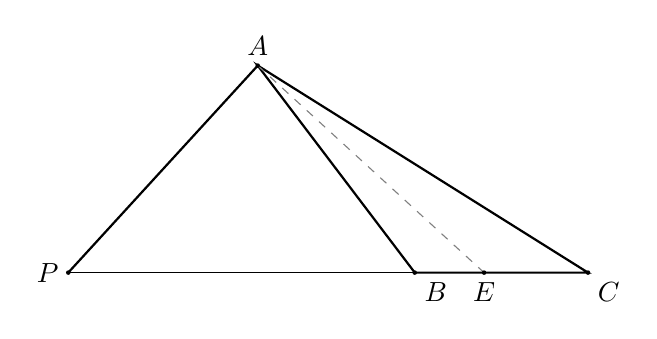
\begin{tikzpicture}[scale=0.55]
    \coordinate (A) at (-3.625,4.78);
    \coordinate (B) at (0,0);
    \coordinate (C) at (4,0);
    \coordinate (P) at (-8,0);
    \coordinate (E) at (1.6,0);
    \draw[thick] (A) -- (B) -- (C) -- cycle;
    \draw (B) -- (P);
    \draw[thick] (A) -- (P);
    \draw[gray,dashed] (A) -- (E);
    \fill (A) circle (1.5pt);
    \fill (B) circle (1.5pt);
    \fill (C) circle (1.5pt);
    \fill (P) circle (1.5pt);
    \fill (E) circle (1.5pt);
    \node[above] at (A) {$A$};
    \node[below right] at (B) {$B$};
    \node[below right] at (C) {$C$};
    \node[left] at (P) {$P$};
    \node[below] at (E) {$E$};
\end{tikzpicture}
\end{center}
Garis putus-putus $AE$ adalah garis bagi dalam,
tegak lurus garis bagi luar $AP$.
\end{proof}

\section{Lemma Incenter-Excenter}

\begin{theorem}[Incenter-Excenter Lemma]
Misalkan $I$ incenter dan $I_A$ $A$-excenter segitiga $ABC$.
Jika garis bagi sudut $A$ memotong lingkaran luar lagi di $M$, maka
\[ MB = MI = MC = MI_A. \]
Dengan kata lain, $M$ adalah titik tengah busur $BC$
yang tidak memuat $A$, sekaligus pusat lingkaran melalui
$B$, $I$, $C$, dan $I_A$.
\end{theorem}
\begin{proof}
Tulis $\angle A = 2\alpha$, $\angle B = 2\beta$.
Karena $M$ titik tengah busur $BC$,
$\angle MBC = \angle MAC = \alpha$. Maka
\[ \angle MBI = \angle MBC + \angle CBI = \alpha + \beta. \]
Di sisi lain, $\angle MIB$ adalah sudut luar segitiga $ABI$ di $I$:
\[ \angle MIB = \angle IAB + \angle IBA = \alpha + \beta. \]
Jadi segitiga $MBI$ sama kaki dengan $MB = MI$;
argumen simetris memberi $MC = MI$.
Untuk $I_A$: garis $BI$ dan $BI_A$ saling tegak lurus
(garis bagi dalam dan luar), jadi $\angle IBI_A = 90^\circ$.
Titik $M$ terletak pada sisi miring $II_A$ (semuanya pada garis bagi $A$)
dengan $MB = MI$, jadi $M$ titik tengah $II_A$ dan $MI_A = MI$.
\end{proof}

\begin{example}
Buktikan bahwa $M$ pada lemma di atas adalah titik tengah segmen $II_A$
dan segiempat $IBI_AC$ siklis berpusat $M$.
\end{example}
\begin{proof}[Solusi]
Titik $I$ di dalam lingkaran luar sedangkan $I_A$ di luar,
jadi ruas $II_A$ memotong lingkaran tepat di $M$.
Karena $MI = MI_A$ menurut lemma, $M$ titik tengah $II_A$.
Kesamaan $MB = MI = MC = MI_A$ mengatakan keempat titik
$B$, $I$, $C$, $I_A$ berjarak sama dari $M$.
\begin{center}
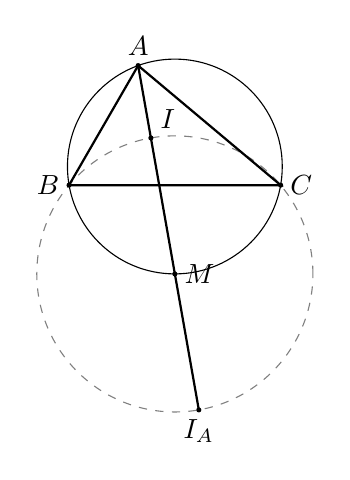
\begin{tikzpicture}[scale=0.62]
    \coordinate (O) at (0,0);
    \coordinate (A) at (-0.752,2.067);
    \coordinate (B) at (-2.167,-0.382);
    \coordinate (C) at (2.167,-0.382);
    \coordinate (I) at (-0.491,0.585);
    \coordinate (M) at (0,-2.2);
    \coordinate (Ia) at (0.491,-4.985);
    \draw (O) circle (2.2);
    \draw[gray,dashed] (M) circle (2.828);
    \draw[thick] (A) -- (B) -- (C) -- cycle;
    \draw[thick] (A) -- (Ia);
    \fill (A) circle (1.5pt);
    \fill (B) circle (1.5pt);
    \fill (C) circle (1.5pt);
    \fill (I) circle (1.5pt);
    \fill (M) circle (1.5pt);
    \fill (Ia) circle (1.5pt);
    \node[above] at (A) {$A$};
    \node[left] at (B) {$B$};
    \node[right] at (C) {$C$};
    \node[above right] at (I) {$I$};
    \node[right] at (M) {$M$};
    \node[below] at (Ia) {$I_A$};
\end{tikzpicture}
\end{center}
\end{proof}

\section{Panjang Garis Singgung}

\begin{lemma}[Panjang garis singgung ke excircle]
Misalkan $B_1$ dan $C_1$ titik singgung $A$-excircle
pada perpanjangan $AB$ dan $AC$, dan $s$ setengah keliling $ABC$. Maka
\[ AB_1 = AC_1 = s. \]
Akibatnya, jika $T_a$ titik singgung pada $BC$, maka
\[ BT_a = s - c \quad\text{dan}\quad CT_a = s - b. \]
\end{lemma}
\begin{proof}
Dua garis singgung dari satu titik sama panjang, jadi $AB_1 = AC_1$,
$BB_1 = BT_a$, dan $CC_1 = CT_a$. Maka
\begin{align*}
AB_1 + AC_1 &= (AB + BB_1) + (AC + CC_1) \\
&= (AB + BT_a) + (AC + CT_a) \\
&= AB + AC + BC = 2s.
\end{align*}
Karena keduanya sama dan jumlahnya $2s$, masing-masing bernilai $s$.
Dari $BB_1 = s - c$ dan $CC_1 = s - b$ didapat akibatnya.
\end{proof}

\begin{example}
Segitiga $ABC$ dengan $BC = 14$, $CA = 13$, $AB = 15$.
Tentukan pembagian sisi $BC$ oleh titik singgung $A$-excircle.
\end{example}
\begin{proof}[Solusi]
Setengah kelilingnya
\[ s = \frac{14 + 13 + 15}{2} = 21. \]
Menurut lemma,
\[ BT_a = s - c = 21 - 15 = 6, \qquad
CT_a = s - b = 21 - 13 = 8. \]
\begin{center}
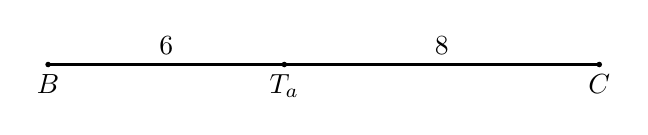
\begin{tikzpicture}[scale=0.5]
    \coordinate (B) at (0,0);
    \coordinate (T) at (6,0);
    \coordinate (C) at (14,0);
    \draw[thick] (B) -- (C);
    \foreach \p in {B,T,C} \fill (\p) circle (2pt);
    \node[below] at (B) {$B$};
    \node[below] at (T) {$T_a$};
    \node[below] at (C) {$C$};
    \node[above] at (3,0) {$6$};
    \node[above] at (10,0) {$8$};
\end{tikzpicture}
\end{center}
\end{proof}

\begin{example}
Misalkan $D$ titik pada sisi $BC$.
Buktikan bahwa $AB + BD = DC + CA$ jika dan hanya jika
$D$ adalah titik singgung $A$-excircle.
\end{example}
\begin{proof}[Solusi]
Tulis $BD = x$, jadi $DC = a - x$.
Persamaan menjadi
\[ c + x = (a - x) + b, \]
yaitu $2x = a + b - c$, atau $x = s - c$.
Nilai ini tepat $BT_a$ menurut lemma,
dan karena $x$ tunggal, $D = T_a$.
Arah sebaliknya langsung dari nilai $BT_a$ dan $CT_a$.
\end{proof}

\section{Jari-Jari Exradius}

\begin{fact}
Misalkan $L$ luas segitiga $ABC$ dan $r_a$ jari-jari $A$-excircle. Maka
\[ r_a = \frac{L}{s - a}, \]
dan analog $r_b = L/(s - b)$, $r_c = L/(s - c)$.
Alasannya luas bertanda: $L$ sama dengan jumlah luas $AI_AB$ dan $AI_AC$
dikurangi luas $AI_ABC$, yaitu
\[ L = \frac12 r_a c + \frac12 r_a b - \frac12 r_a a
= r_a(s - a). \]
\end{fact}

\begin{example}
Segitiga $13$-$14$-$15$ pada contoh sebelumnya:
tentukan jari-jari $A$-excircle jika $a = BC = 14$.
\end{example}
\begin{proof}[Solusi]
Luasnya menurut Heron
\[ L = \sqrt{21 \cdot 7 \cdot 8 \cdot 6} = 84. \]
Akibatnya
\[ r_a = \frac{84}{21 - 14} = \frac{84}{7} = 12. \]
\end{proof}

\section{Homoteti dan Titik Nagel}

\begin{fact}
\istilah{Homoteti}{homothety} berpusat $A$ memetakan lingkaran dalam
ke $A$-excircle, karena keduanya menyinggung kedua sinar garis $AB$
dan $AC$. Homoteti positif ini memetakan titik puncak suatu lingkaran
ke titik puncak lingkaran lainnya.
\end{fact}

\begin{example}
Misalkan $A_0$ titik singgung lingkaran dalam dengan $BC$,
$A'_0$ antipode-nya (ujung diameter yang lain),
dan $A_a$ titik singgung $A$-excircle dengan $BC$.
Buktikan $A$, $A'_0$, $A_a$ segaris.
\end{example}
\begin{proof}[Solusi]
Garis singgung di $A'_0$ sejajar $BC$ (keduanya tegak lurus diameter
$A_0A'_0$), dengan lingkaran dalam di bawahnya.
Peta garis singgung ini oleh homoteti adalah garis singgung excircle
yang sejajar $BC$ dengan excircle di bawahnya, yaitu garis singgung
di $A_a$. Jadi peta $A'_0$ adalah $A_a$,
sehingga $A$, $A'_0$, $A_a$ segaris (segaris dengan pusat homoteti).
\begin{center}
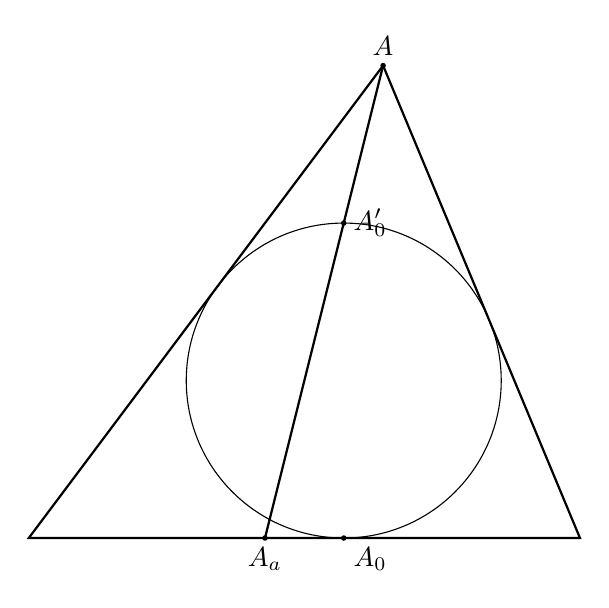
\begin{tikzpicture}[scale=0.5]
    \coordinate (A) at (9,12);
    \coordinate (B) at (0,0);
    \coordinate (C) at (14,0);
    \coordinate (I) at (8,4);
    \coordinate (A0) at (8,0);
    \coordinate (Ap0) at (8,8);
    \coordinate (Aa) at (6,0);
    \draw[thick] (A) -- (B) -- (C) -- cycle;
    \draw (I) circle (4);
    \draw[thick] (A) -- (Aa);
    \fill (A) circle (2pt);
    \fill (A0) circle (2pt);
    \fill (Ap0) circle (2pt);
    \fill (Aa) circle (2pt);
    \node[above] at (A) {$A$};
    \node[below right] at (A0) {$A_0$};
    \node[right] at (Ap0) {$A'_0$};
    \node[below] at (Aa) {$A_a$};
\end{tikzpicture}
\end{center}
\end{proof}

\begin{remark}
Garis-garis $AA_a$, $BB_b$, $CC_c$ (titik sudut ke titik singgung
excircle di sisi hadapan) berpotongan di satu titik yang disebut
\istilah{titik Nagel}{Nagel point}.
Buktinya satu baris Ceva dengan panjang garis singgung:
\[ \frac{BT_a}{T_aC} \cdot \frac{CT_b}{T_bA} \cdot \frac{AT_c}{T_cB}
= \frac{s-c}{s-b} \cdot \frac{s-a}{s-c} \cdot \frac{s-b}{s-a} = 1. \]
\end{remark}

\section{Soal Latihan}

\subsection{Garis Bagi Luar dan Panjang Singgung}
\begin{enumerate}

	% Source: jjmo final 2006 number 4 (diterjemahkan ke Bahasa Indonesia)
	% Jawaban: 55 derajat
	\item (JJMO Final 2006)
	Lingkaran dalam segitiga $ABC$ menyinggung sisi $AB$, $BC$, $CA$
	berturut-turut di $D$, $E$, $F$.
	Jika $\angle BAC = 70^\circ$, tentukan $\angle DEF$.

	% Source: osk sma 2010 nomor 11 isian singkat
	% Jawaban: 3:1
	\item (OSK SMA 2010)
	Diberikan segitiga $ABC$; $AC:CB = 3:4$.
	Garis bagi luar sudut $C$ memotong perpanjangan $BA$ di $P$
	($A$ terletak antara $P$ dan $B$).
	Perbandingan $PA:AB$ adalah \dots

	% Source: osk sma 2014 nomor 15 isian singkat
	% Jawaban: 160
	\item (OSK SMA 2014)
	Diberikan segitiga $ABC$ dengan $AB = 360$, $BC = 240$ dan $AC = 180$.
	Garis bagi dalam dan garis bagi luar dari $\angle CAB$ memotong $BC$
	dan perpanjangan $BC$ berturut-turut di $P$ dan $Q$.
	Jari-jari lingkaran yang melalui titik-titik $A$, $P$ dan $Q$ adalah \dots

\end{enumerate}

\subsection{Lemma Incenter-Excenter}
\begin{enumerate}[resume]

	% Source: 8 Outsource K Math/Pra-OSP/Excircle.tex (HMMT 2013, dimodifikasi)
	\item (HMMT 2013)
	Diberikan segitiga $ABC$ dengan $2BC = AB + AC$ dan incenter $I$
	serta lingkaran luar $\omega$.
	Misal $D$ adalah perpotongan $AI$ dan $\omega$ yang bukan $A$.
	Buktikan bahwa:
	\begin{enumerate}
		\item $I$ adalah titik tengah $AD$,
		\item $OI$ tegak lurus dengan $AI$, dengan $O$ pusat $\omega$.
	\end{enumerate}

	% Source: emc junior 2014 number 3 essay (diterjemahkan ke Bahasa Indonesia;
	% redaksi dilengkapi: AB tak sama dengan AC agar D terdefinisi, dan E di
	% antara D dan F, karena tanpa syarat posisi E dapat menjadi excenter,
	% bukan incenter; garis AB/AC maksudnya garis, bukan segmen)
	\item (EMC Junior 2014)
	Diberikan segitiga $ABC$ dengan $AB \ne AC$.
	Garis bagi luar dan garis bagi dalam $\angle CAB$ memotong garis $BC$
	berturut-turut di $D$ dan $E$.
	Misalkan $F$ titik pada sisi $BC$ sehingga $E$ terletak di antara $D$
	dan $F$. Lingkaran luar segitiga $ADF$ memotong garis $AB$ dan $AC$
	berturut-turut di $I$ dan $J$.
	Misalkan $N$ titik tengah $IJ$ dan $H$ kaki dari $E$ ke $DN$.
	Buktikan bahwa $E$ adalah incenter dari segitiga $AHF$.

	% Source: jjmo final 2010 number 4 (diterjemahkan ke Bahasa Indonesia)
	\item (JJMO Final 2010)
	Diberikan segitiga $ABC$. Lingkaran $\Gamma$ melalui $B$ dan $C$
	memotong sisi $AB$ dan $AC$ (tidak termasuk titik ujung) berturut-turut
	di $D$ dan $E$, dan berlaku $AD + AE = BC$.
	Misalkan $I$ incenter segitiga $ABC$.
	Jika garis $BI$ dan $CI$ memotong $\Gamma$ berturut-turut di $P$
	(selain $B$) dan $Q$ (selain $C$),
	buktikan bahwa $A$, $I$, $P$, $Q$ konsiklis.

\end{enumerate}

\subsection{Jari-Jari dan Homoteti}
\begin{enumerate}[resume]

	% Source: osk sma 2009 versi 2 nomor 11 isian singkat
	% Jawaban: 5/2
	\item (OSK SMA 2009)
	Misalkan pada suatu segitiga $ABC$, $r$ menyatakan panjang jari-jari
	lingkaran dalamnya, $r_a$ menyatakan panjang jari-jari lingkaran
	singgung luar yang menyinggung sisi $BC$, $r_b$ yang menyinggung sisi
	$CA$, dan $r_c$ yang menyinggung sisi $AB$.
	Jika $r = 1$, $r_a = 2$, $r_b = 3$, dan $r_c = 6$,
	maka panjang jari-jari lingkaran luarnya adalah \dots

	% Source: smo 2014 senior round 2 (diterjemahkan ke Bahasa Indonesia;
	% notasi pusat excircle diseragamkan menjadi I_a)
	\item (SMO 2014)
	Pada segitiga $ABC$, excircle di hadapan $A$ yang berpusat di $I_a$
	menyinggung sisi $BC$ di $D$.
	Misalkan $M$ titik tengah $BC$ dan $N$ titik tengah $AD$.
	Buktikan bahwa $I_a$, $M$, $N$ segaris.

	% Source: 8 Outsource K Math/Pra-OSP/Excircle.tex (ToT 1999 Autumn A-level)
	\item (ToT 1999)
	Titik $K$, $L$ terletak di sisi $AC$, $BC$ dari segitiga $ABC$
	dan merupakan titik singgung $B$-excircle dan $A$-excircle
	dengan sisi di hadapannya.
	Buktikan garis lurus yang menghubungkan titik tengah $KL$
	dan titik tengah $AB$ akan:
	\begin{enumerate}
		\item membagi keliling $ABC$ menjadi dua bagian yang sama panjang,
		\item sejajar dengan garis bagi dalam $\angle ACB$.
	\end{enumerate}

	% Source: aime 2019 I problem 11 (diterjemahkan ke Bahasa Indonesia)
	% Jawaban: 20
	\item (AIME I 2019)
	Pada $\triangle ABC$, sisi-sisinya memiliki panjang bulat dan $AB = AC$.
	Lingkaran $\omega$ berpusat di incenter $\triangle ABC$.
	Andaikan excircle yang menyinggung $\overline{BC}$ bersinggungan dalam
	dengan $\omega$, sedangkan dua excircle lainnya keduanya bersinggungan
	luar dengan $\omega$.
	Tentukan nilai terkecil yang mungkin dari keliling $\triangle ABC$.

\end{enumerate}

\subsection{Esai Pilihan}
\begin{enumerate}[resume]

	% Source: osp sma 2014 nomor 2 esai
	\item (OSP SMA 2014)
	Diberikan segitiga $ABC$ lancip dengan $AB < AC$.
	Lingkaran singgung luar dari segitiga $ABC$ yang berlawanan terhadap
	$B$ dan $C$ berturut-turut berpusat di $B_1$ dan $C_1$.
	Misalkan $D$ titik tengah dari $B_1C_1$.
	Misalkan pula $E$ adalah titik perpotongan dari $AB$ dan $CD$,
	serta $F$ adalah titik perpotongan dari $AC$ dan $BD$.
	Jika $EF$ memotong $BC$ di titik $G$,
	buktikan bahwa $AG$ adalah garis bagi dari $\angle BAC$.
	(Lingkaran singgung luar yang berlawanan terhadap $B$ didefinisikan
	sebagai lingkaran yang menyinggung $AC$ di segmennya serta menyinggung
	$AB$ dan $BC$ di perpanjangannya.)

	% Source: osp sma 2025 nomor 3 esai
	\item (OSP SMA 2025)
	Pada segitiga $ABC$, misalkan $D$ titik tengah ruas garis $AB$
	dan $E$ titik pada sisi $BC$.
	Misalkan garis yang melalui $E$ dan sejajar $AB$ memotong garis bagi
	$\angle ACB$ di titik $P$.
	Misalkan juga $I$ titik pusat lingkaran dalam $ABC$ dan $J$ pusat
	lingkaran singgung luar dari segitiga $ABC$ yang menyinggung sisi $CA$
	(bukan perpanjangan sisi $CA$).
	Garis $DJ$ memotong sisi $CA$ di titik $F$.
	\begin{enumerate}
		\item Buktikan bahwa garis $IF$ sejajar dengan $AB$.
		\item Buktikan bahwa garis $AP$, $BJ$, dan $EF$ berpotongan di satu titik.
	\end{enumerate}

	% Source: pmo national written 2022 number 6 essay (diterjemahkan ke Bahasa Indonesia)
	\item (PMO 2022)
	Pada $\triangle ABC$, misalkan $D$ titik pada sisi $BC$ sehingga
	$AB + BD = DC + CA$.
	Garis $AD$ memotong lingkaran luar $\triangle ABC$ lagi di titik
	$X \ne A$.
	Buktikan salah satu garis singgung persekutuan lingkaran luar
	$\triangle BDX$ dan $\triangle CDX$ sejajar $BC$.

	% Source: imo shortlist 2012 geometry problem 1 (diterjemahkan ke Bahasa Indonesia)
	\item (IMO SL 2012)
	Pada segitiga $ABC$, titik $J$ adalah pusat excircle di hadapan $A$.
	Excircle ini menyinggung sisi $BC$ di $M$, dan garis $AB$ dan $AC$
	berturut-turut di $K$ dan $L$.
	Garis $LM$ dan $BJ$ berpotongan di $F$, dan garis $KM$ dan $CJ$
	berpotongan di $G$.
	Misalkan $S$ titik potong garis $AF$ dan $BC$,
	dan $T$ titik potong garis $AG$ dan $BC$.
	Buktikan bahwa $M$ adalah titik tengah $ST$.

	% Source: OrtikEx_Materi.tex dan Pelatda OSN SMA 2026 (All-Russian MO 2022 Grade 9 P2;
	% diterjemahkan ke Bahasa Indonesia)
	% Jawaban: 1/3
	\item (All-Russian 2022)
	Diberikan segitiga $ABC$ dengan incenter $I$ dan $A$-excenter $J$.
	Lingkaran $\omega_b$ berpusat di $O_b$ melalui $B$ dan menyinggung
	garis $CI$ di $I$.
	Lingkaran $\omega_c$ berpusat di $O_c$ melalui $C$ dan menyinggung
	garis $BI$ di $I$.
	Misalkan $O_bO_c$ dan $IJ$ berpotongan di $K$.
	Tentukan rasio $IK/KJ$.

	% Source: osn sma 2018 nomor 8 esai
	\item (OSN SMA 2018)
	Misalkan $I$ dan $O$ masing-masing menyatakan titik pusat lingkaran
	dalam dan lingkaran luar dari segitiga $ABC$.
	Lingkaran singgung luar $\omega_A$ dari segitiga $ABC$ menyinggung
	sisi $BC$ di $N$ serta menyinggung perpanjangan sisi $AB$ dan $AC$
	masing-masing di $K$ dan $M$.
	Jika titik tengah dari ruas garis $KM$ berada pada lingkaran luar
	segitiga $ABC$, buktikan bahwa $O$, $I$, dan $N$ segaris.

\end{enumerate}

\end{document}
